\section{RunOff Application}
\label{sec:sprint2-app}
For the second sprint there was focus on getting the application to display a map for the user with their selected route drawn onto it, preferably with \ac{GPS} tracking. The implementation of the application was hindered by the choice of \ac{IDE} seeing as Android Studio is an early alpha product and certain bugs made it exceedingly difficult to integrate the Google Maps \ac{API}. Thus the work done consisted mainly of failed attempts at integration concluding with porting the project to another \ac{IDE} and then integrating the maps and drawing the route.

\subsection{User Interface}
The interface for the majority of the application remained largely unchanged in this sprint, however a new screen was added with a map that displayed the chosen route. As the emphasis is on competing in a race the map covers the entire screen in the application, centring on the starting point of the route and zoomed in enough to give an overview of the route. The user can then zoom in more themselves by double-tapping the screen. A mock-up of the interface is shown in \autoref{fig:mapMock}.

\begin{figure}[!ht]
	\begin{center}
		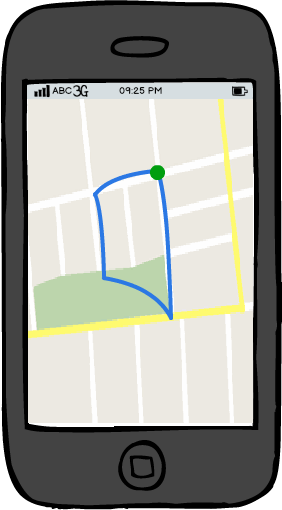
\includegraphics[scale=0.4]{img/mapMock.png}
		\caption{Map User Interface Mockup}
		\label{fig:mapMock}
	\end{center}
\end{figure}

\subsection{Implementation}
The implementation of the map functionality was done by creating a new activity, called \texttt{RunProgress}, to display the route and in the future the progress of the race. This activity was started when the user selected a route from the list of available routes in the \texttt{PickRoute} activity. The \texttt{PickRoute} forwards the chosen route's information to the \texttt{RunProgress} activity. The chosen route, among other things, contains an encoded polyline which is decoded and added to the map. As well, the coordinates of the starting waypoint of the route is utilized in centring the map's camera on the starting point of the route. The implementation is fairly trivial code-wise and will not be discussed further. In \autoref{fig:runProgressV1} the resulting map, with a small route drawn, is shown.

\begin{figure}[!ht]
	\begin{center}
		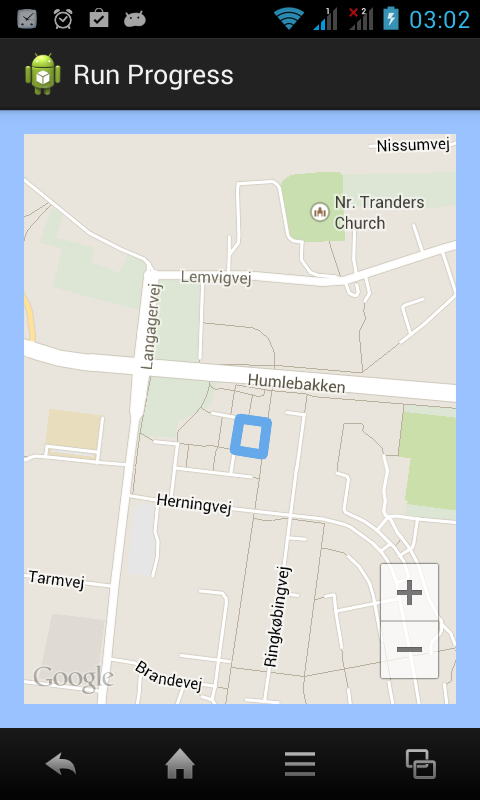
\includegraphics[scale=0.4]{img/runProgressV1.png}
		\caption{Map User Interface}
		\label{fig:runProgressV1}
	\end{center}
\end{figure}

\subsection{Testing}
As all the activity does at the moment is create a map and draw a polyline based on the route's information, a single unit test was written which starts the activity, asserts that the map is created and that the number of coordinates used to draw the polyline are correct when compared to the ones received. The code coverage report can be seen in \autoref{tab:emma2}

\begin{table}[!ht]
	\centering
	\begin{tabular}{| c | c | c | c |}
		\hline
		\textbf{Class} & \textbf{Method} & \textbf{Block} & \textbf{Line} \\ \hline
		100 \% (16/16) & 80 \% (50/62) & 70 \% (900/1287) & 75 \% (219/292) \\
		\hline
	\end{tabular}
	\caption{EMMA Coverage Results}
	\label{tab:emma2}
\end{table}
